\chapter{The Alpha experiment}
\label{ch:apparatus}

\ALPHA (Antihydrogen Laser Physics Apparatus) is an international collaboration, based at the Antiproton Decelerator (AD) facility at CERN, whose origin can be traced back to the ATHENA collaboration. ATHENA was the first experiment to produce low-energy antihydrogen, by merging cold trapped antiproton and positron plasmas in a Penning-Malmberg trap, and reported this milestone in 2002 \cite{Amoretti2002}, together with the competing ATRAP collaboration. This production scheme, still at the core of every antihydrogen experiment operating today, made it possible to study the antihydrogen formation rate, its dependence on the antiproton and positron plasma temperature and density, and to develop the annihilation-vertex imaging techniques on which later trapping and spectroscopy measurements would rely. Once antihydrogen production was established, the natural next objective became the magnetic trapping of the neutral anti-atoms, a goal that required an apparatus fundamentally different from ATHENA's. Around 2005, some members of the ATHENA collaboration regrouped to form the \ALPHA collaboration, built around a new octupole-based neutral atom trap (see Sec. \ref{sec:antihydrogensynthesis}), while ATHENA itself was decommissioned.

In the two decades since, \ALPHA has produced a steady sequence of milestones in antihydrogen physics, each opening the way to the next:

\begin{itemize}
\item \textbf{2010} -- first magnetic trapping of antihydrogen atoms \cite{ALPHA:2010oyp};
\item \textbf{2011} -- confinement of trapped antihydrogen for up to 1000 seconds, demonstrating that anti-atoms could survive long enough for spectroscopy \cite{Amole:2011cvt};
\item \textbf{2012} -- first resonant, microwave-induced quantum transition driven in trapped antihydrogen, the spin-flip technique underlying the hyperfine measurements discussed in this thesis \cite{ALPHA:2012kaf};
\item \textbf{2016/2017} -- observation of the 1S-2S transition \cite{Ahmadi:2016fyz} and first measurement of the ground-state hyperfine spectrum \cite{ALPHA:2017fsh} of antihydrogen;
\item \textbf{2021} -- first laser cooling of trapped antihydrogen atoms, using the Lyman-$\alpha$ (1S-2P) transition \cite{Baker:2021ncj};
\item \textbf{2023} -- first direct observation, with the ALPHA-g apparatus, of the effect of gravity on the motion of antimatter \cite{Anderson:2023wnq};
\item \textbf{2025} -- Be$^{+}$-assisted cooling routinely enables the simultaneous trapping of more than 15000 antihydrogen atoms \cite{Akbari:2025mli};
\item \textbf{2026} -- a four parts-per-million measurement of the ground-state hyperfine splitting \cite{ALPHA:2026lbu}, the topic of this thesis.
\end{itemize}

This progression reflects three intertwined threads of development: increasingly sophisticated plasma and antihydrogen manipulation techniques, colder and more numerous trapped samples, and ever more precise diagnostic tools (magnetometry, detection, laser and microwave spectroscopy), all of which are described in the remainder of this chapter.

\section{Antiproton decelerator facility at CERN (AD)}

The CERN Antiproton Decelerator (AD, \cite{theantiprotondecelerator}) is the dedicated facility for low-energy antiproton physics and, together with ELENA, constitutes the accelerator infrastructure underlying current antimatter precision experiments. Its development should be viewed in continuity with the earlier LEAR program (1982–1996), where key techniques for antiproton deceleration, beam cooling, and precision measurements were established (\cite{Poth1990}, \cite{CarliCaspers2000}). Following LEAR’s shutdown, the AD was commissioned in 1999 to provide a reproducible and experiment-oriented source of antiprotons at energies compatible with trapping and atomic-physics methods. In the standard production chain, primary protons from the Proton Synchrotron are directed onto a fixed Iridium target \cite{PhysRevAccelBeams.19.073402}; the secondary antiprotons are collected and subsequently decelerated through staged cycles with cooling to reduce emittance and momentum spread prior to extraction. The AD is capable of decelerating antiproton bunches down to 5.3 MeV.

A substantial extension of this scheme was introduced with ELENA (Extra Low ENergy Antiproton ring), integrated into the AD complex in the late 2010s and used for physics operation in the early 2020s \cite{Bartmann2018}. ELENA further decelerates antiprotons from the AD extraction energy down to approximately 100 keV and improves the transverse and longitudinal beam characteristics relevant for capture in Penning traps and antihydrogen formation apparatuses. Operationally, this stage increases the trapping efficiency of antiprotons for the various experiments, improves antihydrogen production in ALPHA, and enables more effective sharing of antiproton delivery across multiple experimental zones.

\begin{figure}[!hbtp]
\centering
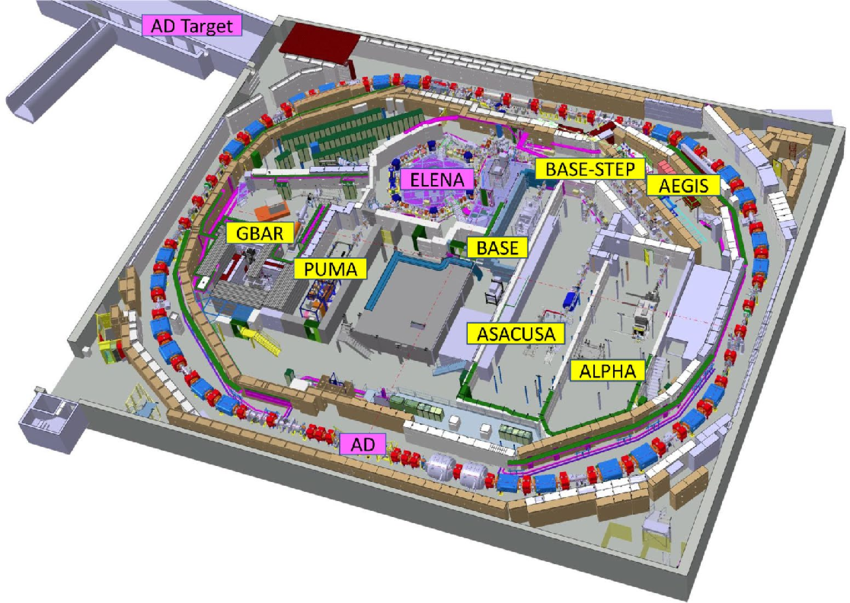
\includegraphics[width = 0.75\textwidth]{figures/chapter 2/Overview-on-the-AD-ELENA-facility-The-AD-with-a-circumference-of-183-m-constrains-the.png}
\caption{Scheme of the Antimatter Factory facility, with the Antiproton decelerator and the ELENA ring. 7 experiments are currently operating, with the ALPHA experimental area on the right side of the diagram.}
\end{figure}

The historical evolution of the facility is directly reflected in the scientific output of the AD era. Early AD operation enabled the first production of cold antihydrogen (ATHENA and ATRAP, 2002 \cite{Amoretti2002}). Subsequent experiments established trapped-antihydrogen techniques and high-precision spectroscopy (notably in the ALPHA and ASACUSA programs), while complementary Penning-trap measurements (e.g., BASE) provided stringent comparisons of antiproton and proton properties, including charge-to-mass ratio and magnetic moment \cite{Ulmer2015}. In parallel, antiprotonic-atom studies by the ASACUSA collaboration, methodologically connected to the LEAR tradition, continued to contribute to precision bound-state tests. More recently, dedicated experiments (AEgIS, GBAR, ALPHA-g) have extended the scope of the AD program to gravitational observables of neutral antimatter \cite{Aegisproposal}, \cite{GBAR:2011fij} \cite{ALPHA:2013skd}. In this sense, the AD/ELENA complex is not merely a beam-delivery system, but a structured platform that links accelerator performance parameters (energy, emittance, duty cycle, and extraction conditions) to the achievable precision and systematic control of contemporary antimatter measurements.

\section{The ALPHA experiment}

The \ALPHA (Antihydrogen Laser Physics Apparatus) is one of the 7 experiments located at the Antimatter Factory facility at CERN. \ALPHA focuses on antihydrogen physics, and aims to measure energy levels of the antihydrogen atoms, comparing antihydrogen with hydrogen, as well as gravitational acceleration measurements on antimatter. The \ALPHA apparatus, whose schematic overview is shown in figure \ref{fig:AlphaSchematicOv},\begin{sidewaysfigure}[hp]
\centering
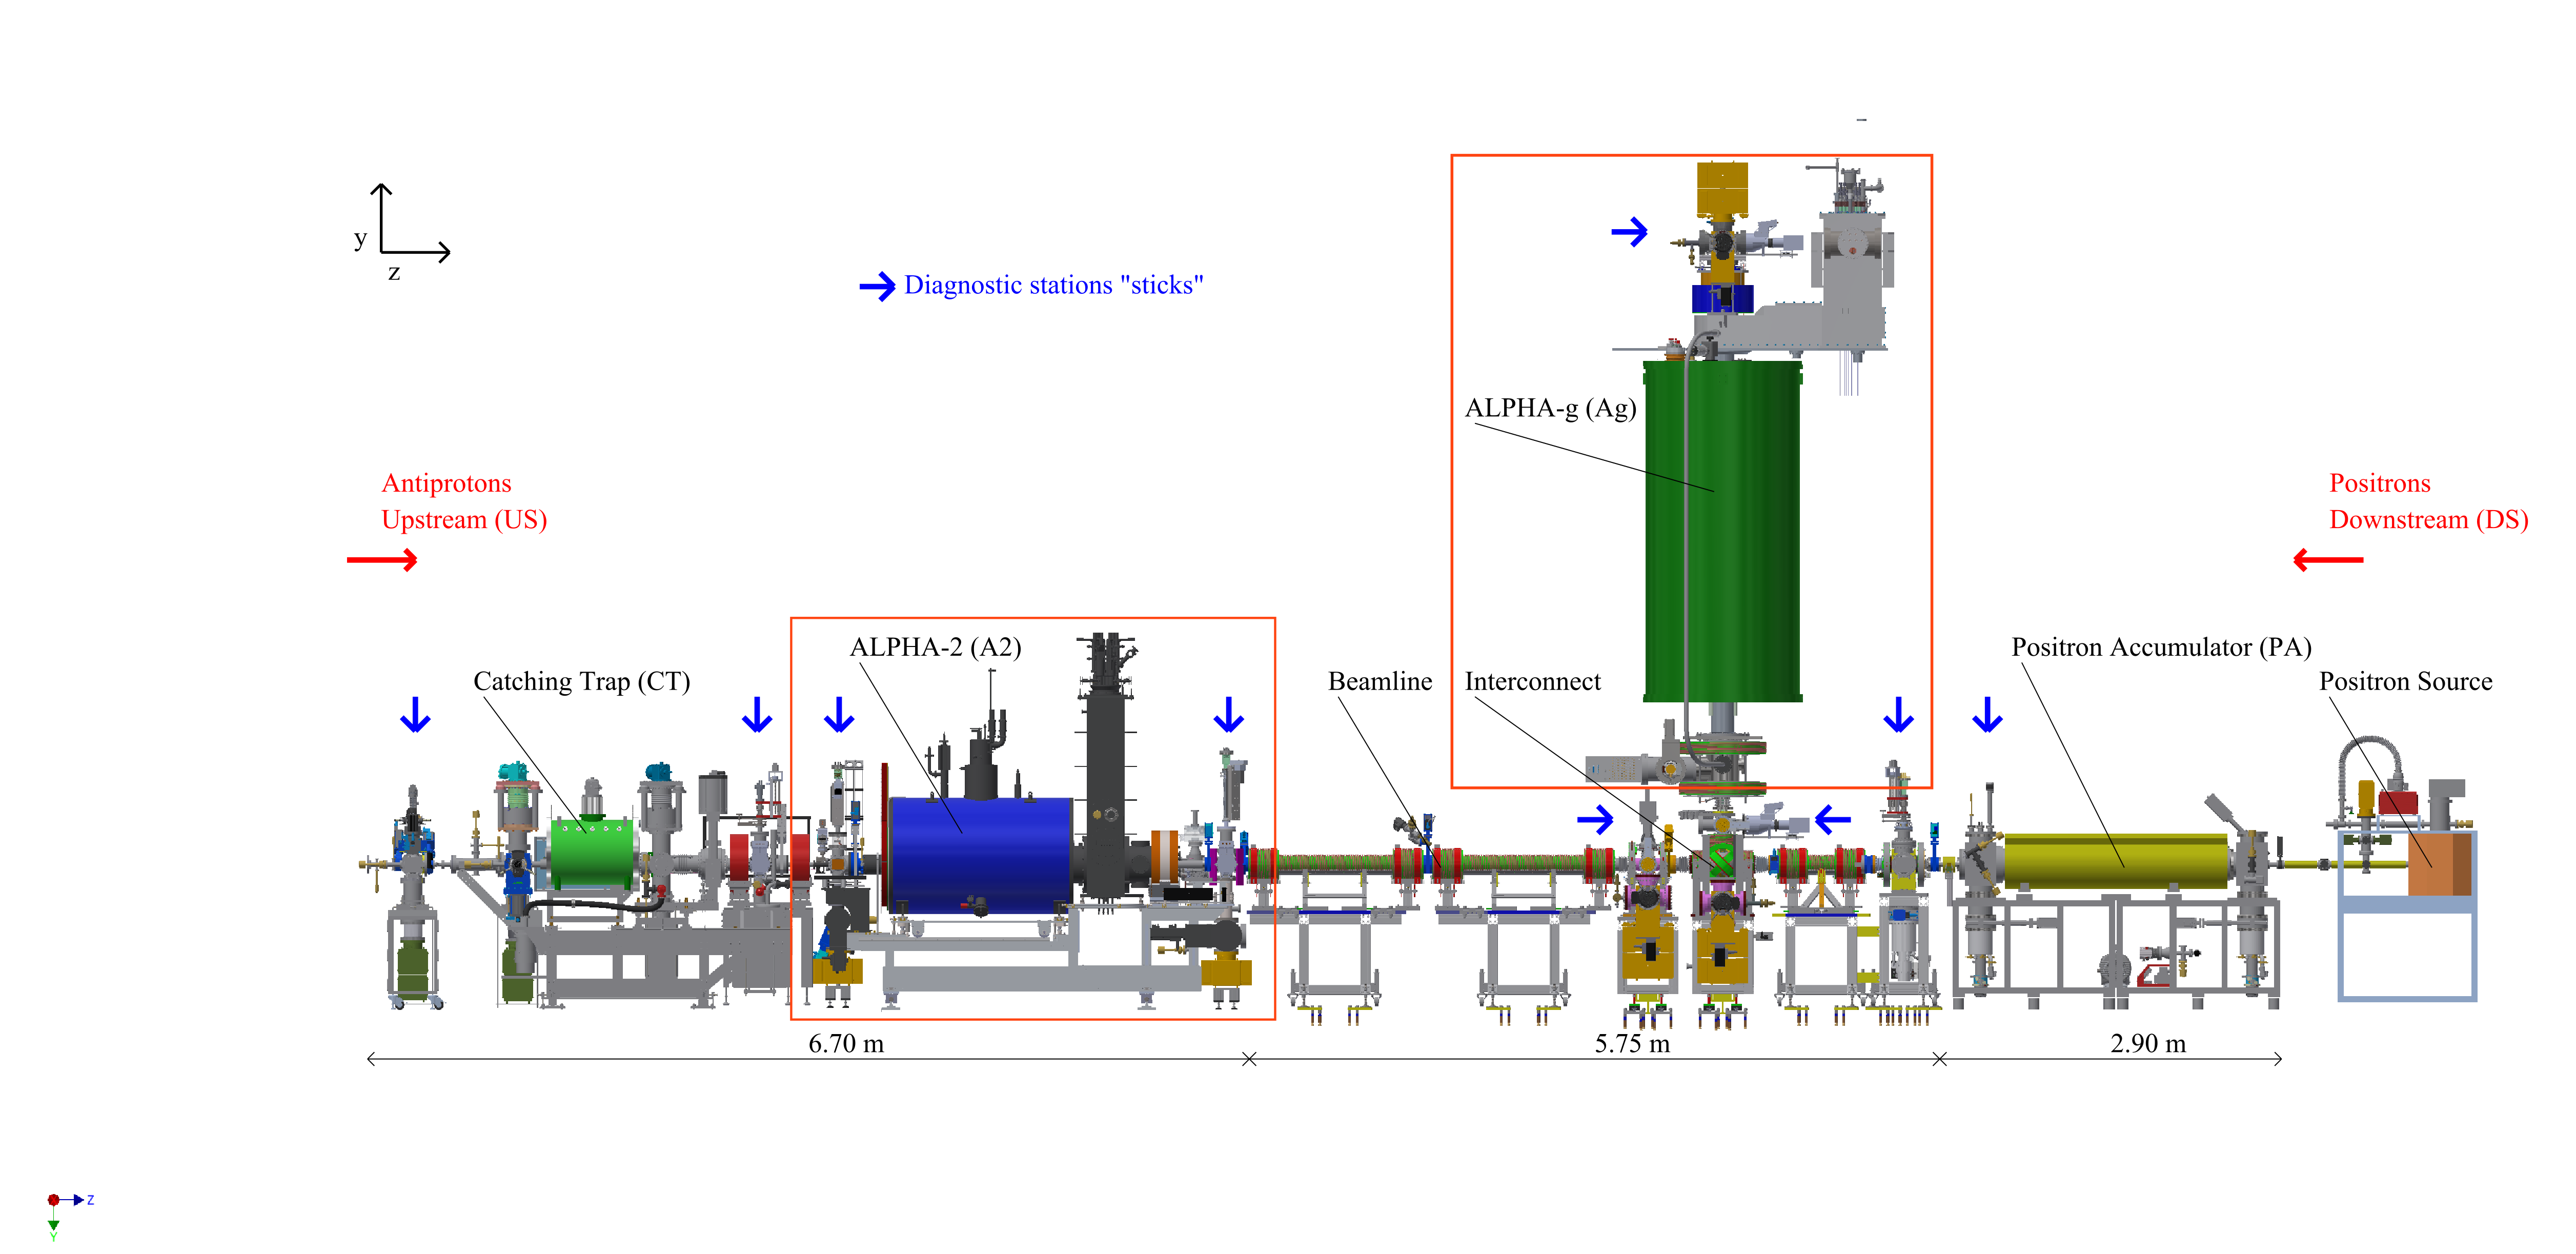
\includegraphics[width = \textwidth]{figures/chapter 2/ALPHA_full.png}
\caption{Schematic overview of the ALPHA apparatus. The antiprotons are received from the antiproton decelerator beam-line, that is connected to the experiment from the left side (Upstream), and collected by the Catching Trap (CT) for plasma manipulation and cooling. The positron plasma comes from a radioactive source from the right side of the image. The two sections of the experiment are clearly visible: the vertical ALPHA-g apparatus, to measure gravitational acceleration on antimatter, and the ALPHA-2 apparatus, designed for spectroscopy. This image is a reproduction from thesis \cite{Singh:2025uuo}}.
\label{fig:AlphaSchematicOv}
\end{sidewaysfigure}
is designed to synthesize, by manipulating antiproton and positron plasma, antihydrogen atoms, that are confined by the interaction of the magnetic momentum with an external magnetic field ( $\approx$ \SI{ 1 }{\tesla} ), provided by a superconducting solenoid and several mirror coils. The antihydrogen synthesis is achieved by manipulating antiproton and positrons plasma with a set of Penning-Malmberg traps, which are constituted by electrodes that can be controlled independently, and are used to design electric potential for plasma manipulation. The Penning traps are a common tool in non-neutral plasma and trapped ion physics, which is used to manipulate plasma to obtain desired characteristics. In \ALPHA three Penning traps are available, that have different purpose: the catching trap (designed for antiprotons capture), the positron accumulator trap (for positron plasma) and the ALPHA2 Penning-Malmberg trap (for antihydrogen synthesis).
 In the following section, a general overview of the experiment section and how antihydrogen is synthesized is presented, with particular focus on the implications for the measurement that is the topic of this thesis.

\section{Penning trap, physics principles}

A Penning trap confines charged particles using a combination of static electric and magnetic fields \cite{DEHMELT196853}. A uniform axial magnetic field  $\vec{B} = B \hat{z}$ provides radial confinement: any transverse motion of a charged particle is bent into a circular orbit by the Lorentz force, preventing radial escape. Axial confinement, which the magnetic field alone cannot provide, is instead achieved with a static electric field generated by a set of cylindrical electrodes: the end electrodes are held at a potential of the same sign as the trapped charge, while a central electrode is held at the opposite potential, creating an electrostatic potential well along the trap axis that reflects the particle back toward the centre whenever it approaches either end.

The resulting particle motion is a superposition of three independent oscillations: a fast circular motion in the plane perpendicular to $\vec{B}$, known as the cyclotron motion; a slower axial oscillation along $\hat{z}$ inside the electrostatic well; and a slow azimuthal drift around the trap axis, known as the magnetron motion, arising from the $\vec{E} \times \vec{B}$ drift induced by the radial component of the trapping electric field. In practice, ALPHA traps are cylindrically symmetric, multi-electrode versions of this basic design — Penning–Malmberg traps — in which a stack of many short cylindrical electrodes, rather than just three, allows the trapping potential to be reshaped dynamically along the trap axis, enabling the plasma manipulations (compression, transport, splitting, merging) needed for the experiment.
Malmberg and deGrassie \cite{PhysRevLett.35.577} extended the single-particle Penning trap concept to the confinement of large numbers of like-charged particles, or non-neutral plasmas, in which collective electrostatic interactions can no longer be neglected. In this regime, the plasma settles into a rigid-rotor equilibrium about the trap axis, with radial confinement governed by the plasma's total angular momentum rather than by single-particle dynamics alone. The practical advantage of a multi-electrode design is that the axial potential can be reshaped purely electronically: by varying the voltages on successive electrodes, a confining well can be deepened, split, merged, or translated along the trap axis, allowing the plasma to be transported and manipulated without ever losing axial confinement. These capabilities make the Penning–Malmberg trap, rather than the single-particle Penning trap, the design of choice for the antiproton and positron plasma manipulations performed throughout the ALPHA apparatus.

\section{The positron accumulator}

The positron accumulator at ALPHA is that part of the apparatus (shown in the upper part of Fig. \ref{fig:AlphaSchematicOv}) that is designed to accumulate positrons for antihydrogen synthesis. The main mechanism of the apparatus, which is based on cooling/trapping with buffer nitrogen gas, was first designed by Surko and Murphy in 1992 \cite{MurphySurko1992}.
The positrons are provided by a strong radioactive source, which contains $^{22}Na$ sodium, which decays into $^{22}Ne$ through $\beta^{+}$ decay. The isotope has a half-life of 2.6 \textit{y}, which makes it possible to have a stable and reproducible positron plasma for the experimental operation.

Positrons immediately released from the sodium source have energies of the order of units of $keV$, and must be slowed down in order to be trapped and manipulated for antihydrogen synthesis. A fraction of the emitted positrons (the ones emitted with a direction aligned with the accumulator) passes through a solid Neon moderator, which slows positrons down to less than $100 \; eV$ of kinetic energy. Only a fraction of the emitted positrons (efficiency about 1\%) are able to cross the Neon moderator; afterwards they are collected in the positron accumulator volume, a multi-stage device filled with cold low-pressure nitrogen gas (see Fig. \ref{fig:PositronAccumulator}). Nitrogen acts as a cooling mechanism through elastic collisions (the nitrogen electronic excitation cross-section has a prominent resonance around $9 \; eV$), decreasing positron energies further:

\begin{equation}
e^{+} + N_{2} \rightarrow e^{+} + N^{*}_{2}
\end{equation}

while a Penning trap surrounding the plasma ensures confinement with a potential well. The Penning trap which controls the potential is divided in three stages, and the last allows the application of a \textit{rotating} electric field for plasma size compression. A more detailed description of the design of the positron accumulator and its principles is reported in \cite{10.1063/1.859558} and \cite{10.1063/1.870693}. During normal operation, the accumulations last for \SI{100}{\second}, after which roughly 20 million positrons are accumulated. After the accumulation phase, the buffer nitrogen gas is pumped out to minimize the vacuum contamination along the beam-line, and the positron cloud is moved along the beamline by lowering the potential barrier (see Fig \ref{fig:PositronAccumulator}, second panel). Positron plasma transfer along the beam line reduces the available quantity for antihydrogen synthesis to roughly $3.7$ million, which is a target number before the antihydrogen synthesis.

\begin{figure}[!hbtp]
\centering
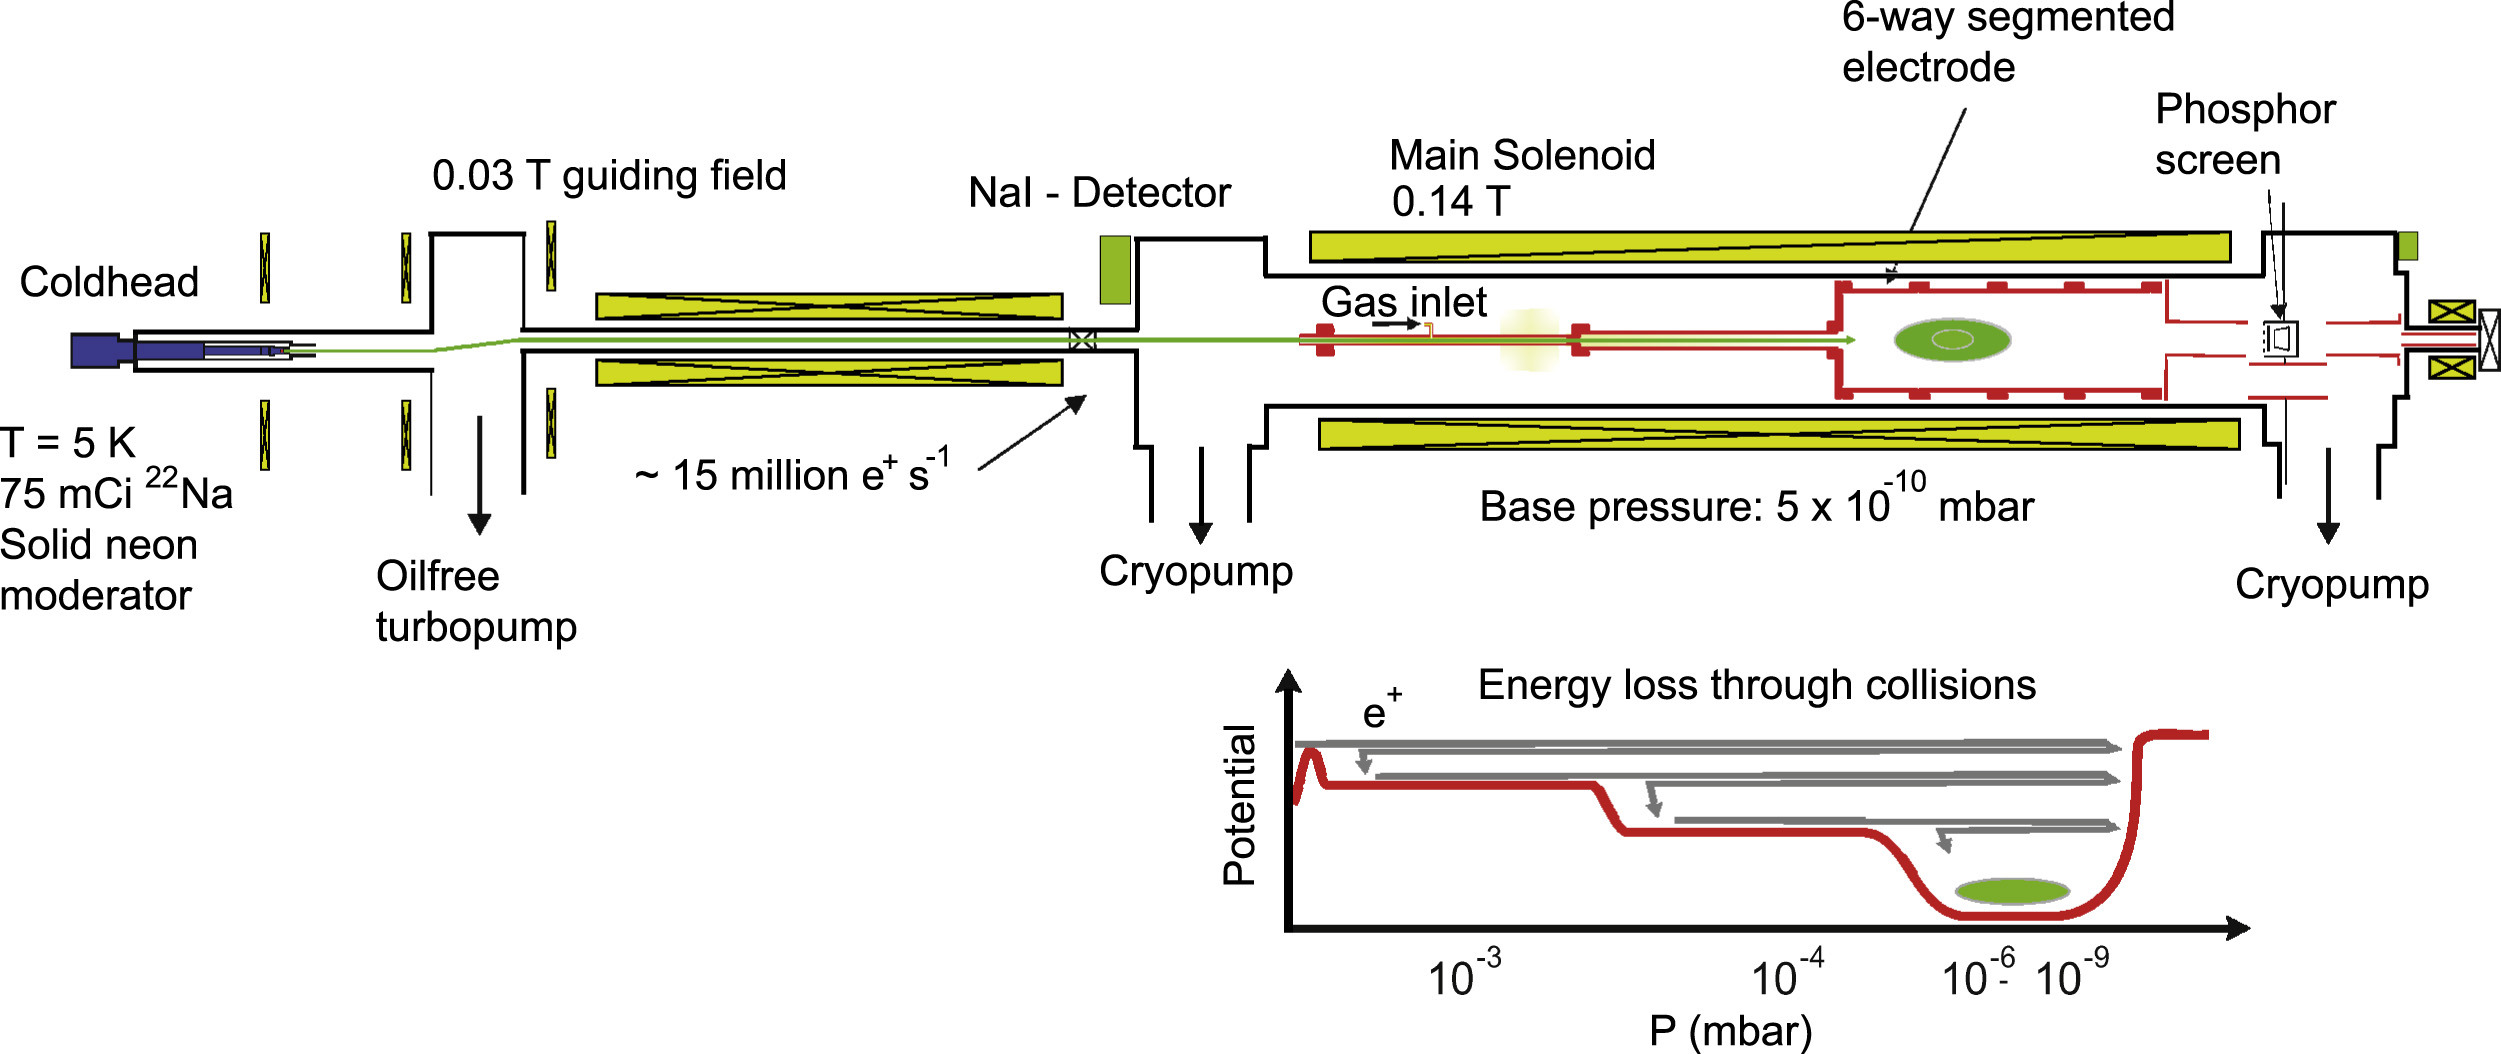
\includegraphics[width = \textwidth]{figures/chapter 2/Positron-acc-scheme.jpg}
\caption{Positron beamline and positron accumulator schematic illustration. The lower panel in the figure represents the axial electric field potential of the Penning trap. The grey arrows represent an example positron trajectory and collisions lead to accumulation of positrons in the third stage of the accumulator volume. This figure is taken from \cite{AMOLE2014319}}
\label{fig:PositronAccumulator}
\end{figure}


\section{The catching trap}

The catching trap (CT) is the device designed for the first stage preparation of antiproton plasma in \ALPHA; it receives antiproton bunches from the ELENA ring at an energy of about \SI{100}{\kilo \eV}. CT is constituted by a cryogenic Penning-Malmberg trap with a solenoidal field of \SI{3}{\tesla}, located after the ELENA distribution beamline for ALPHA, and it is shown in the left part of the scheme in Fig. \ref{fig:AlphaSchematicOv} (labeled as \textit{CT}, shown in light green). The antiprotons arriving at the catching trap are first subjected to an energy selection, as they pass through transverse aluminum foils (degraders) that reduce their kinetic energy \cite{fabbrisiara}. The surviving fraction of antiprotons are captured in the catching trap between two fast-acting high-voltage electrodes. These high-voltage electrodes are energized once the antiproton bunch enters the catching trap volume, in rapid succession raising confining potentials on the "right" and "left" sides, so that the bunch becomes trapped between them. The potential configuration allows only antiprotons with kinetic energies below $4.5 \; keV$ to remain confined, and the more energetic fraction leaks out.
The antiproton plasma is subjected to several manipulations inside the catching trap. Firstly, the antiprotons are cooled down by using pre-loaded cold electrons in the trap volume. Electrons are useful since they emit Larmor radiation due to their motion inside the trap. The power emitted can be written as:

\begin{equation}
P = \frac{q^{2} a^{2}}{6 \pi \epsilon_{0} c^{3}}
\end{equation}

Here $a$ is the local acceleration experienced by an electron. During their motion inside the trap, electrons tend to emit photons and reduce their available kinetic energy, reaching a much lower temperature with respect to the antiprotons delivered to the experiment. While this cooling mechanism is very efficient for light electrons, it is negligible for antiprotons, since their mass is 2000 times larger \footnote{Assuming a Maxwell-Boltzmann distribution for the charged plasma, it is possible to derive the characteristic cooling time $\tau$ as $\tau = \frac{9 \pi \epsilon_{0} m^{3} c^{3}}{2 q^{4} B^{2}}$, to make explicit the dependence on the mass of the particle species.}. Therefore, antiproton cooling is achieved by elastic collisions with pre-loaded electrons, until the two particle species reach equilibrium at the same temperature.
Sympathetic cooling with electrons typically lasts for \SI{20}{\second}, after which the electrons are removed by quickly lowering and raising the potential well. This procedure, referred to as \textit{ekick}, is made fast enough such that very few antiprotons are lost while the majority of the electrons is removed, and it is repeated three times interspersed with cooling periods, leaving a cold antiproton plasma. During the cooling phases, rotating voltages are applied to the segmented electrodes of the trap, so that the mixed antiproton-electron plasma undergoes radial compression, to minimize losses during transfer toward ALPHA-2 (or ALPHA-g) trap.
 Typically, about half a million antiprotons are trapped and cooled with this technique from a single bunch of the \AD, and about $\simeq 350000$ \commento{mmm, quindi però bisogna aggiornarsi rispetto ai mixing triggers, i numeri della tesi di maria non sono aggiornati} are efficiently transferred to the ALPHA-2 left trap (also commonly known as the re-catching trap), where the same cooling mechanism is repeated with another pre-loaded electron plasma. This transfer stage is typically the dominant source of antiproton loss in the whole preparation chain, and ultimately limits the antihydrogen production rate. Once the second cooling stage is completed, the antiproton plasma is placed at the center of the atom trap, for antihydrogen production. 

\section{The ALPHA2 Penning-Malmberg trap}

Until now, the Penning-Malmberg trap has been introduced for the manipulation of charged particles in the experiment. Although such devices are fundamental for charged plasma manipulation and formation of anti-atoms, they cannot be used to trap neutral particles. The ALPHA-2 neutral trap is a hybrid device specifically designed for antihydrogen formation and confinement, that superimposes a Penning-Malmberg trap, used to prepare and manipulate charged antiproton and positron plasma, with an octupole magnet and a series of solenoids. By doing so, it is possible to generate inhomogeneous magnetic field profiles that can exploit the dipole moment of neutral particles or atoms to achieve confinement. 
The ALPHA2 trap is divided in three segments with two different radii. The left and right side traps are made of 7 electrodes of \SI{30}{\milli \meter} each, and are used to "re-catch" antiprotons from the catching trap and positrons from the accumulator (the smaller radius allows for larger magnetic field, improving cooling rates). The central, wider trap is made of 13 cylindrical electrodes, with a larger inner radius of \SI{45}{\milli \meter}, and it is instead used for antihydrogen synthesis and confinement. Optical access for the laser system is provided both through off-axis laser ports along the trap and through vacuum windows at the diagnostic stations located at either end of the apparatus.

\begin{figure}[!hbtp]
\centering
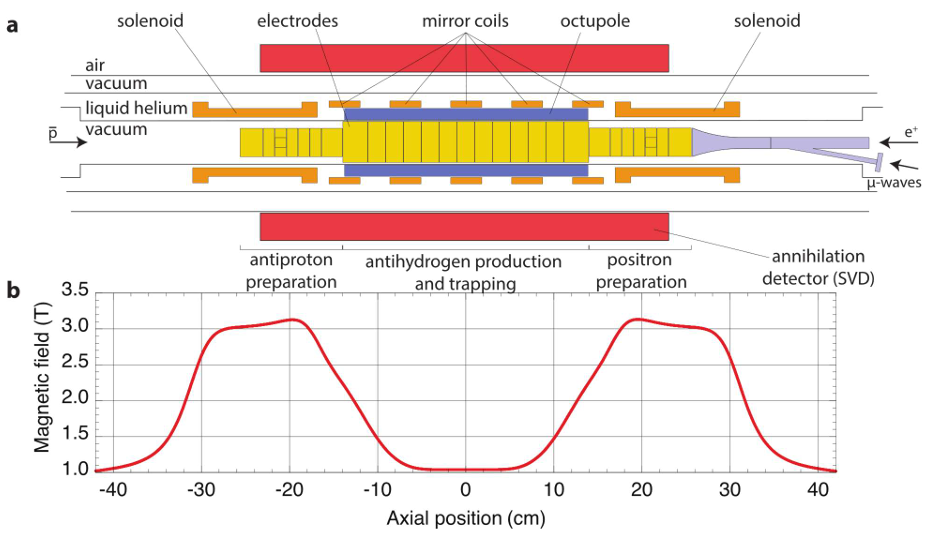
\includegraphics[width=\textwidth]{figures/Bfield_with_tramscheme_draftpaper.png}
\caption{Scheme of the ALPHA2 Penning–Malmberg trap (top) and on-axis magnetic field profile for axial confinement of the antihydrogen atoms (bottom).}
\label{fig:TrapScheme}
\end{figure}

In its ground state, the magnetic moment of antihydrogen originates almost entirely from the positron spin, so that atoms with spin anti-aligned to the local field are drawn towards regions of lower field magnitude ("low-field seekers"), while aligned atoms are repelled. By combining an octupole magnet, chosen over a quadrupole or hexapole configuration to maximize the volume over which the field minimum is flat, with a set of mirror coils providing axial confinement, a local minimum in the magnetic field magnitude is created at the center of the trap. The resulting well has a depth on the order of \SI{0.5}{ \kelvin}, which is dictated by practical magnet current and operational limitations. Only a small fraction of the antihydrogen atoms formed is cold enough to remain trapped. An illustration of the ALPHA2 neutral trap is shown in Fig. \ref{fig:TrapScheme}. The neutral trap magnetic field is shaped, along the trap axis, like a shallow "bathtub," with a minimum of \SI{1.1}{\tesla} located at the center of the Penning–Malmberg trap (coinciding with the synthesis region) and rising to about \SI{3.3}{\tesla} near the segmented electrodes at either end. This field configuration is produced by superconducting solenoid pairs at each end of the trap ("mirror" magnets, providing axial confinement) combined with an octupole magnet (providing radial confinement); the octupole is typically operated at 900 A during antihydrogen synthesis. A set of additional mirror coils allows fine adjustment of the field profile to be as axially flat as possible across the synthesis region, maximizing the trapping volume. The preparation and combination of the antiproton and positron plasmas that leads to the actual formation of antihydrogen within this trap is described separately in the following section.


\subsection{Synthesis of antihydrogen} \label{sec:antihydrogensynthesis}

Once the antiproton and positron plasmas have each been individually prepared, cooled, and transferred into the neutral trap (or, in the ALPHA-g apparatus), they are held in separate potential wells until the final stage of the plasma manipulation cycle: mixing. 

The two plasmas are initially located at the two smaller Penning traps (left and right side traps) and are moved into the central wider trap. The central trap electrodes produce an electric potential that is designed to both trap antiproton and positron clouds, as shown in Fig \ref{fig:Antihydrogen-formation}. The two plasmas are gradually brought closer by lowering the potential barrier between them. Before the barrier is fully removed, the positron plasma undergoes a final evaporative cooling stage, achieved by lowering the potential wall on the side opposite the antiprotons and allowing the most energetic positrons to escape; the remaining positrons re-thermalize at a lower temperature. Then, the potential is further decreased so that antiproton and positron clouds finally merge. This last phase consists of lowering the final separation barrier such that antiprotons are moved into the positron plasma, while positrons are free to escape to the left and get through the antiproton cloud. This mechanism enhances positron evaporative cooling, which acts throughout the mixing phase, lowering the plasma temperature, which ultimately enhances antihydrogen formation.

\begin{figure}[hbtp]
\centering
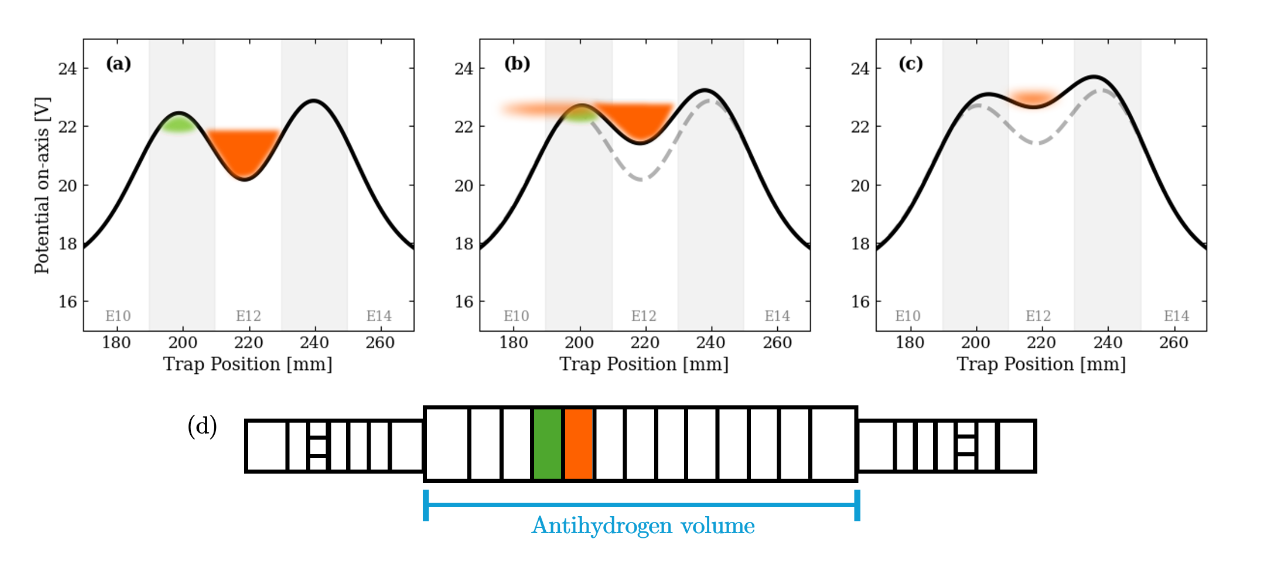
\includegraphics[width = \textwidth]{figures/chapter 2/Antihydrogen_formation.png}
\caption{ This picture illustrates the slow merge technique used to synthesize antihydrogen. Positron (orange cloud) and antiproton plasma (green cloud) are initially in separate locations as shown in \textbf{(a)}. By slowly raising the central potential minimum, antiproton and positron clouds meet, and antihydrogen is synthesized through three-body recombination \textbf{(b)}. The mixing phase ends with the final potential state shown in \textbf{(c)}, with some positrons still trapped, and used for diagnostic purposes (i.e., to measure the final positron temperature after mixing). The duration of the mixing phase is typically in the range of a few seconds, and it is a parameter tuned to maximize antihydrogen production. This figure is reproduced from \cite{goncalves:2025uuo} }
\label{fig:Antihydrogen-formation}
\end{figure}

Antihydrogen is formed by a three-body recombination process. The process consists of two positrons simultaneously getting close to an antiproton: one positron binds with the antiproton and forms antihydrogen, while the other is ejected away carrying the excess energy:

\begin{equation}
\overline{p} + e^{+} + e^{+} \rightarrow \overline{H} + e^{+}
\end{equation}

This channel is favored compared to two-body recombination. The reason is that for the two-body recombination process, the kinetic energy of the formed anti-atom is comparable to that of the antiproton participating in the process. The resulting kinetic energy of the anti-atom is comparable to the thermal energy of the antiprotons, which makes it difficult for the atom to be cold enough to be confined by the magnetic field minimum (of the order of \SI{0.5}{\kelvin}). Three-body recombination, by contrast, can in principle produce antihydrogen without depositing this excess energy into the atom's kinetic energy, making it the dominant source of trappable atoms under ALPHA's experimental conditions. Of all antihydrogen atoms formed during a mixing cycle, only the fraction with kinetic energy below the trap depth remains confined once the mixing sequence ends; the rest escape and annihilate on the surrounding electrode walls. At the end of the mixing, the magnets can be de-energized, to release confined antihydrogen, or kept energized while other mixing cycles are performed in succession, in order to accumulate a larger sample of anti-atoms (stacking technique).

\subsection{Beryllium cooling}

The Beryllium cooling system constitutes a fundamental milestone for the \ALPHA experiment, since it has improved antihydrogen formation from a few atoms to hundreds of atoms, also reducing the final antihydrogen temperature distribution. This technique has been established in \ALPHA in 2024, and it is extensively described in Maria Gomes Goncalves's thesis \cite{goncalves:2025uuo}, and results were published in Nature Communications (\cite{Baker:2021ink}). During the 2024/2025 experimental campaign, further improvements of the Beryllium cooling system allowed a record accumulation of over 15000 trapped antihydrogen atoms in 7 hours \cite{Akbari:2025mli}.

A well-established solution in non-neutral plasma physics is sympathetic cooling: a species that can be cooled directly (the coolant), typically via laser cooling, is mixed with the species to be cooled (the target), and energy is transferred between the two populations through Coulomb collisions. This approach was first demonstrated in 1986 by cooling $^{198}Hg^{+}$ ions through collisions with laser-cooled $^{9}\text{Be}^{+}$ in a Penning trap, and its use to cool positron plasmas via laser-cooled $Be^{+}$ ions was subsequently demonstrated in 2003. At ALPHA, this technique has been extended to routinely cool millions of positrons to cryogenic temperatures directly within the Penning–Malmberg trap used for antihydrogen production.

$^{9}\text{Be}^{+}$ is selected as a coolant species because it is the lightest ion with an electronic structure suitable for direct laser cooling, minimizing the mass ratio between the target species and the coolant, which maximizes the energy exchange through collisions.

The $\text{Be}^{+}$ ions are produced in situ by pulsed laser ablation of a solid beryllium target — a method chosen for its compatibility with the geometry and vacuum requirements of the cryogenic trap, avoiding the need for an external atomic beam source — and are then laser-cooled on a cycling optical transition (wavelength \SI{313}{\nano \meter}) before being merged with the positron plasma. As cooling proceeds, Coulomb collisions transfer energy from the positrons to the colder $\text{Be}^+$ ions; however, as the plasma cools, the heavier ions migrate radially outward relative to the positrons due to centrifugal separation, reducing the spatial overlap between the two species and eventually limiting the minimum achievable positron temperature to a few kelvin, well above the Doppler limit of the $\text{Be}$ ions themselves. This limiting temperature depends on the number of ions used, initially decreasing with a larger coolant population before plateauing once centrifugal separation sets in.

This "Final Laser Cooling" step, performed immediately before mixing, has become the standard technique for preparing cold positron plasmas at ALPHA, replacing purely evaporative cooling schemes. The resulting increase in positron phase-space density has translated into a substantially higher antihydrogen yield, with $\text{Be}^{+}$ assisted cooling reported to increase the number of trapped antihydrogen atoms per synthesis cycle by roughly a factor $\approx 10$ between the 2023 and 2024 experimental runs.

\section{Electron cyclotron resonance technique (ECR)} \label{sec:ECRtecnique}

The ECR (Electron Cyclotron Resonance) is a powerful sensing technique, developed in the \ALPHA collaboration, to measure the on-axis magnetic field in a Penning-Malmberg trap. This technique has been developed in 2014 \cite{Amole:2014lna} and refined by \textit{Eric Hunter} \cite{Hunter_2020}, and exploits the interaction between a small electron plasma and the external magnetic field, combined with microwave radiation injected into the trap, to determine the magnetic field magnitude at a given axial position. Accurate measurements of the magnetic field are required for precision measurements of the atomic spectra as well as the gravitational acceleration of antihydrogen in ALPHA-g.

The measurement relies on a Penning--Malmberg trap, in which a large electron plasma reservoir ($2$--$3\times10^{7}$ electrons) is first prepared and stabilized in temperature, density and particle number via strong-drive regime evaporative cooling (SDREVC). Small target plasmas, containing as few as $N_T \sim 1500$ electrons, are then repeatedly extracted from the reservoir by manipulating the electrode potentials, moved to a dedicated heating well, and further evaporatively cooled (see figure \ref{fig:SchemeECR}). This reservoir-based approach allows more than 100 target plasmas to be produced from a single loading of the electron source, enabling a complete frequency scan in about one minute and avoiding the systematic drifts associated with repeated source operation.
Assuming the z parallel to the trap axis, each target plasma is moved along the axis to the location of interest by tuning the electrode potentials. Then, the plasma is kept in place by the electrode potential (also experiencing a magnetic field $B\hat{z}$) and it is illuminated with a microwave pulse (typically $100\,\mathrm{ms}$ long) whose frequency $F$ is swept across a range of values. When $F$ approaches the electron cyclotron frequency $f_c = eB/2\pi m_e$, the plasma absorbs energy from the microwave field and is heated. The resulting plasma temperature is measured destructively: the downstream confinement potential is slowly lowered at a fixed rate, and the arrival rate of the escaping electrons at a microchannel plate (MCP) detector is recorded. Since the most energetic electrons escape first as the barrier is lowered, the time history of the MCP signal directly encodes the plasma temperature, which is extracted through a fit to the expected escape-rate model.

A scan of $T$ versus $F$ typically reveals not a single resonance but a series of heating peaks, spaced by the electron axial bounce frequency $f_z$ and further split into subpeaks separated by the plasma (magnetron) rotation frequency $f_r$. These sidebands arise because the oscillating electron motion in the trapping well and its slow rotation around the trap axis modulate the microwave field seen by the electron, shifting the resonance condition away from the bare cyclotron frequency. Among these substructures, the $l=-2$ subpeak of the central ($m=0$) resonance is identified as the one whose frequency is, to first order, independent of both the bounce and rotation frequencies, and is therefore taken as the true cyclotron resonance used to extract $B$ through inversion of $B = (2\pi m_e/e)\,f_c$.

Using this method, ALPHA reports absolute magnetic field measurements with an accuracy better than $1\,\mathrm{ppm}$, and a relative precision of $26\,\mathrm{ppb}$ when combining several bounce-frequency scans, dominated respectively by environmental field drifts (of thermal origin, linked to the electron source) and by residual plasma-charge and finite-temperature systematic shifts.

\begin{figure}[hbtp]
\centering
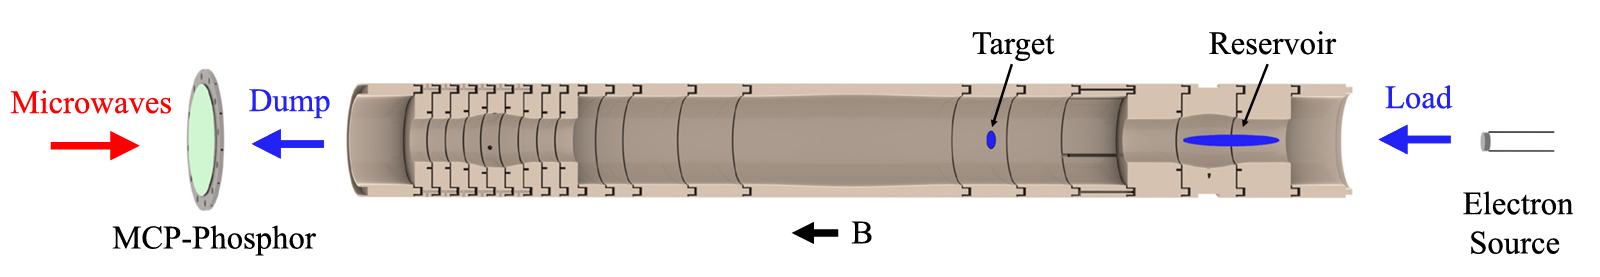
\includegraphics[width=\textwidth]{figures/chapter 2/ECR-scheme.png}
\caption{Scheme of ALPHA-2 Penning-Malmberg Trap, with illustration of the main ECR measurement phases (preparation of the plasma reservoir, extraction, microwave heating and dump). The figure is reproduced from \cite{Hunter_2020}}
\label{fig:SchemeECR}
\end{figure}

The ECR technique is actually used in the measurement both for designing the magnetic trapping potential for synthesis of antihydrogen and spectroscopy in ALPHA-2, and furthermore makes it possible to keep track of magnetic field changes by repeating ECR measurements in a time series.


\section{Detection of antiprotons}

The detection of antimatter in the ALPHA2 experiment is made possible with a silicon vertex detector (SVD), designed for the detection of an annihilation once an antihydrogen atom or an antiproton hits the electrodes of the trap. The annihilation products are mainly charged pions $\pi^{\pm}$, and by reconstructing and analyzing the tracks of their passage in the detector, it is possible to extract the vertex of the annihilation, which is the main measurement tool in spectroscopy experiments \cite{ALPHA:2012wlk}.
The detection of antimatter in the ALPHA-2 experiment is made possible with a silicon vertex detector (SVD), designed for the detection of the annihilation that occurs once an antihydrogen atom or an antiproton hits the electrodes of the trap. The detector consists of three concentric layers of double-sided silicon microstrip modules, arranged coaxially around the trap magnets so as to surround the entire synthesis region. The annihilation products are mainly charged pions $\pi^{\pm}$, and by reconstructing and analyzing the tracks left by their passage through the successive silicon layers, it is possible to extract both the spatial position and the timing of the annihilation vertex, with a typical resolution of about 0.5 cm along the trap axis and 0.9 cm radially \cite{Capra:2015ozr}. This vertex reconstruction is the main measurement tool in spectroscopy experiments, and it also allows genuine antiproton annihilations to be distinguished from a background of cosmic-ray events, based on the track topology and timing of the reconstructed events.

\subsection{The ALPHA2 silicon vertex detector}

The silicon vertex detector is a 3-layer detector that is placed around the trap center reaching almost full azimuthal coverage. The scheme of the detector is shown in figure \ref{fig:SVDscheme}. The detector is made of 72 modules, each constituted by 256 p-side and 256 n-side strips. The modules are arranged in two separate sections along the axial direction with three concentric layers of 36 modules each. The choice of a multi-layer detector is driven by the fact that in such a way it is possible to sample three points of the trajectory of a charged pion in its flight, and hence reconstruct the track of the particle, and the annihilation vertex. 

\begin{figure}[hbtp]
\centering
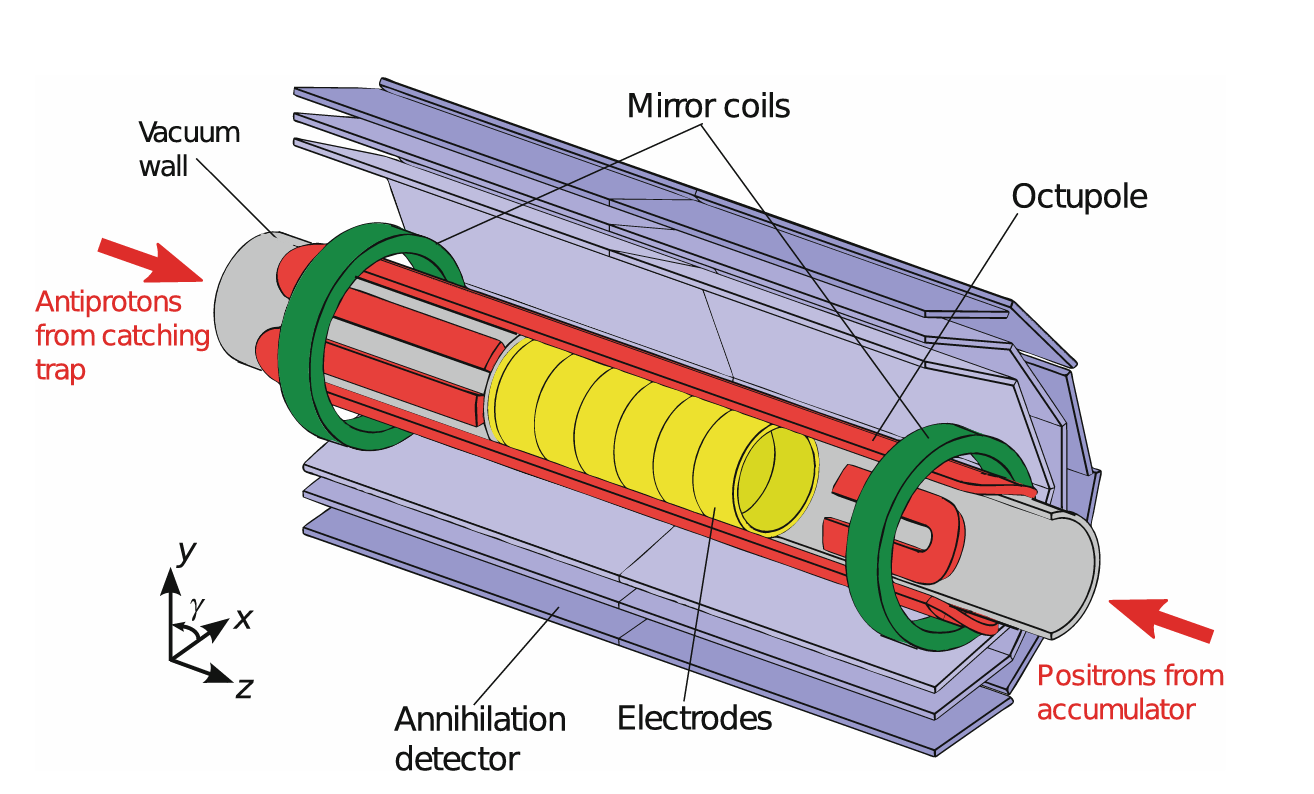
\includegraphics[width = 0.75\textwidth]{figures/chapter 2/Alpha2 Detecor.png}
\caption{Scheme of the ALPHA2 silicon vertex detector (not to scale). The detector is made of 72 modules, that are read out by ASICs. The figure is reproduced from \cite{ALPHA:2012wlk}.} \label{fig:SVDscheme}
\end{figure}

The signals of the detector are constituted by 'hits' in the silicon strips of each module, that are read-out by VA1TA ASIC read-out chips, which control both the read-out and the trigger of an acquisition.
The position information of a hit within a module is achieved by combining the signal information of the p-side and n-side strips of a \textit{hit}, and the passage is localized in the plane of the module.

\begin{figure}[hbtp]
\centering
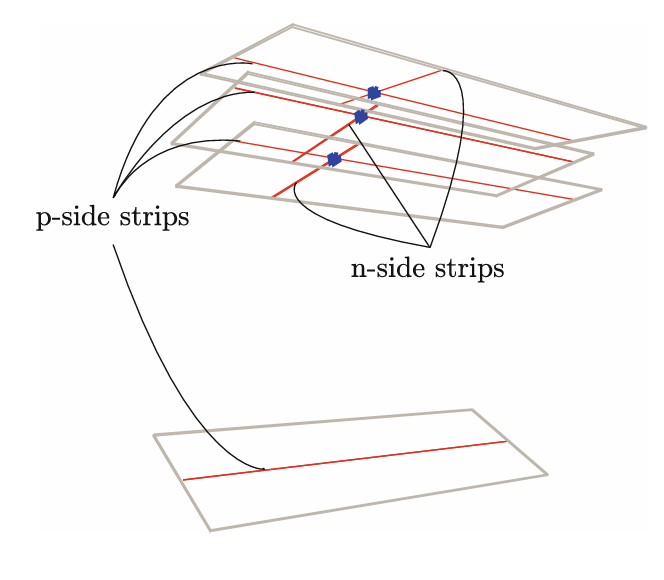
\includegraphics[width = 0.75\textwidth]{figures/chapter 2/Example-of-track.png}
\caption{Example of track and localization of the position of the passage within a module of the detector. The image is reproduced from \cite{Hydomako2013}}
\end{figure}

During an experiment, the main source of background is constituted by cosmic tracks, mainly charged cosmic muons $\mu^{\pm}$, that are recorded by the detector. These energetic cosmic muons travel across the apparatus and are recorded as a single track composed of six hits. The topology of the cosmic events is different from the ones coming from real antiproton or antihydrogen annihilation, hence various pieces of information can be used to discriminate the two cases. This information is combined in a Multi-Variable Analysis (MVA) that is used to effectively suppress the cosmic background to a rate of \SI{37.4}{\milli \hertz}.

\section{Detection of positrons}
\contentof{Qui si può parlare un po' dei burritos, perchè no, come progetto collaterale}

The previous section briefly described the main detector used for antihydrogen detection. Obviously, \ALPHA has several detectors which are used for imaging the plasma or measuring its temperature, etc.
The \ALPHA experiment apparatus is provided with different diagnostic stations, some of which are highlighted in Fig. \ref{fig:AlphaSchematicOv} with blue arrows, which are equipped with Microchannel plates made with phosphor (also known by the abbreviation MCP). The MCP is a two-dimensional detector that can detect electrons, ions, X-rays in vacuum, and it is a common tool in plasma physics. When a charged particle traverses the MCP, it produces a cascade of secondary electrons that produce phosphorescence photons, which are collected by a CCD camera, producing an image of the plasma in the \textit{x,y} plane of the MCP plate. These diagnostic stations are widely used in \ALPHA to study the temperature, size and evolution of the various plasmas (electrons, positrons, antiprotons) along the beamline. They provide good spatial resolution, which allows them to be used for alignment and to benchmark several plasma manipulation techniques. However, although providing spatial information, it is hard to use such detectors to characterize the time structure of the plasma dump when moved along the beamline. In light of this, part of the work of this thesis was dedicated to the development of a system of fast scintillators, placed at several locations along the apparatus, to measure the time distribution of the positron plasma during the various transfers along the trap. The choice of the detector has been made considering that the width of the positron plasma (in terms of time distribution) is expected to be on the order of $\approx$ \SI{10}{\nano \second}, which requires fast detection, namely a detection mechanism that is fast enough so as not to cause signal smearing that would result in a loss of information. Another collateral consideration was driven by the fact that the environment in the proximity of the various beam-line and Penning traps is influenced by magnetic fields that are not shielded. Given these two conditions, photomultiplier technology was rejected and the natural choice was to employ plastic scintillators coupled with silicon photo-multiplier devices. The scintillating material used for this application is the Ej-200, a plastic scintillator made with polyvinyltoluene doped with fluorophores \cite{eljensite}. The scintillating material was selected for being sensitive to gamma rays emitted by positrons, once they annihilate on the plate of an MCP, or on the beamline frame in case of losses. The gamma rays are converted into visible light (blue light $\approx$ \SI{425}{\nano \meter}) that is detectable by SIPMs that are connected via an optical coupler to one side of the scintillating material. The signal produced by the SIPMs is then processed with an OPA354 signal amplifier, in TIA mode (so converting the current signal from the SIPM to a voltage signal). The electronic board that houses the amplifier is custom made, and a scheme can be found in Fig. \commento{qui ci vuole una figura con uno schema, tempo di ottenerla}. The signal output is still analog, and it is sent to Red Pitaya FPGA boards, that are used as the DAQ system. Each Red Pitaya has two input channels, that can acquire independently two signals with a minimum sampling rate of \SI{8}{\nano \second} and a buffer length of 16384, corresponding to a time span of \SI{131.072}{\micro \second}. The Red Pitayas are controlled by an online Python script that continuously monitors the devices, triggers new acquisitions, and saves the data in \textit{.txt} format for further analysis. A separate Python script takes care of analyzing the signals once they are collected, running continuously. The analysis of the signals consists first of a de-noising procedure, where spurious noise is eliminated by applying a low-pass filter with a \SI{9.3}{\mega \hertz} cutoff; hence the offset of the signals is subtracted, and the signal is fitted with an asymmetric Gaussian function, to extract the FWHM, the peak time position, the amplitude and the total area of the signal (which is proportional to the total number of positrons). This information is then recorded on CERN \textit{EOS}, which is a distributed storage system available at CERN. Together with Dr. Samuel Niang, a web application was implemented to make it possible for operators to visualize this information together with signal plots. The web application was implemented using the \textit{NGINX} library, and it is accessible from the CERN local network.


